
%Finite length dipole


\section{Finite Length Dipole}
\subsection{要求}
\noindent 画出不同长度的电偶极子方向图$l=\dfrac{\lambda}{10},\dfrac{\lambda}{4},\dfrac{\lambda}{2},\lambda,\dfrac{3\lambda}{2}$ 

\noindent 选做:

1.计算正弦电流分布的情况下, 不同物理长度偶极子的等效长度.

2.画出任意长度偶极子沿线电流为均匀分布的时候的方向图,并与教材比对.

\subsection{原理及推导}
\subsubsection{考虑电流分布}
\noindent 有限长度且考虑电流分布电偶极子的远场解
\begin{equation}
	E_\theta=\int_{-l/2}^{+l/2}\,\mathrm{d}E_\theta\simeq j\eta\dfrac{ke^{-jkr}}{4\pi r}\sin\theta\left[\int_{-l/2}^{+l/2}\,I_e\left(x',y',z' \right) e^{jkz'\cos\theta}\mathrm{d}z'\right]
\end{equation}
计算积分得到
\begin{equation}
	E_\theta\simeq j\eta\dfrac{I_0e^{-jkr}}{2\pi r}\left[\dfrac{\cos\left(\dfrac{kl}{2}\cos\theta\right)-\cos\left(\dfrac{kl}{2}\right)}{\sin\theta}\right].
\end{equation}


\begin{equation}
	H_\phi\simeq \dfrac{E_\theta}{\eta}\simeq j\dfrac{I_0e^{-jkr}}{2\pi r}\left[\dfrac{\cos\left(\dfrac{kl}{2}\cos\theta\right)-\cos\left(\dfrac{kl}{2}\right)}{\sin\theta}\right].
\end{equation}

由于, 最终需要得到归一化的功率方向图.所以常数项可以直接忽略. 
远场可以视为TEM波,故
\begin{equation}
	P=\dfrac{E^2}{\eta} \simeq \left[\dfrac{\cos\left(\dfrac{kl}{2}\cos\theta\right)-\cos\left(\dfrac{kl}{2}\right)}{\sin\theta}\right]^2.
\end{equation}
编程时亦只关注这一部分. 
\subsubsection{选做: 不考虑电流分布}
不考虑电流分布的时候,电偶极子的远场解简化为
\begin{equation}
	E_\theta=\int_{-l/2}^{+l/2}\,\mathrm{d}E_\theta\simeq j\eta\dfrac{ke^{-jkr}}{4\pi r}\sin\theta\left[\int_{-l/2}^{+l/2}\,I_0e^{jkz'\cos\theta}\mathrm{d}z'\right]
\end{equation}
计算积分得到
\begin{equation}
	E_\theta\simeq\sin\theta\left[ \int_{-l/2}^{+l/2}\,e^{jkz'\cos\theta}\mathrm{d}z' \right] =\dfrac{2\sin\theta\sin \left(\dfrac{kl}{2}\cos\theta\right)}{k\cos\theta}
\end{equation}
\begin{equation}
P\simeq \left[\tan\theta\sin\left(\dfrac{kl}{2}\cos\theta\right)\right]^2
\end{equation}
\subsection{结果与分析}
\subsubsection{方向图与HPBW}
根据图\ref{fig:DP}分析, 随着电偶极子尺寸的增大,方向图越来越瘦,半功率波束宽度也逐渐减小,其定向性越来越好.半功率波束宽度具体见图\ref{fig:DP3dB} .

当$l=1.25\lambda$时候,放大图片,容易观察到,出现了旁瓣. 且随着电偶极子长度的增加,旁瓣越来越大,最后甚至超过主瓣.

\begin{figure}[!ht]
%\small
\centering
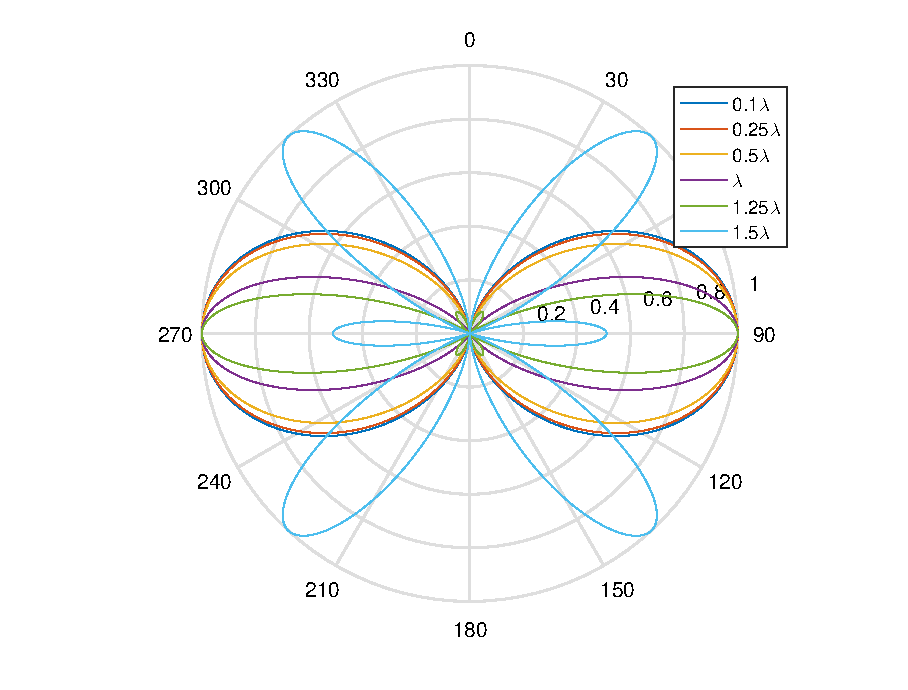
\includegraphics[width=10cm]{DipolePattern.eps}
\caption{DipolePattern} \label{fig:DP}
\end{figure}

\begin{figure}[!ht]
\centering
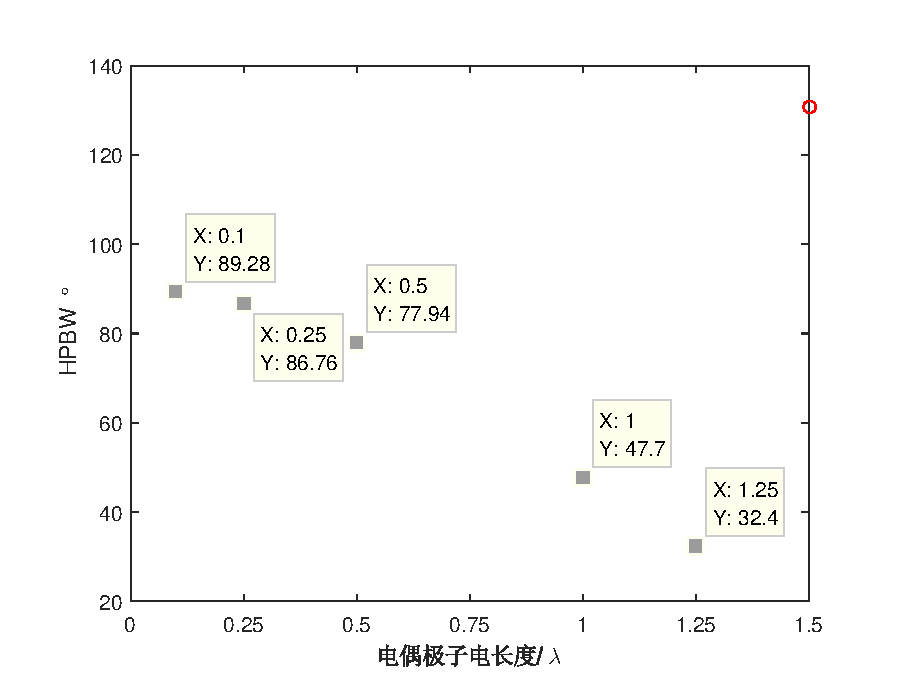
\includegraphics[width=10cm]{Dipole_3dB_beamwidth.eps}
\caption{HalfPowerBeamWidth} \label{fig:DP3dB}
\end{figure}
\subsubsection{选做:不同尺寸电偶极子等效电长度}
结果如表\ref{tab:EQ_L},图\ref{fig:DP_EQ_L} .
\\
\begin{table}[!ht]
\centering
\begin{tabular}{cccccc}
\toprule
实际电长度&0.1 &0.2&0.5&1&1.5\\
\midrule
等效电长度&0.0078&0.0304&0.1592&0.3183&0.4775\\
\bottomrule
\end{tabular}
\caption{等效电长度} \label{tab:EQ_L}
\end{table}


\begin{figure}[!ht]
\centering
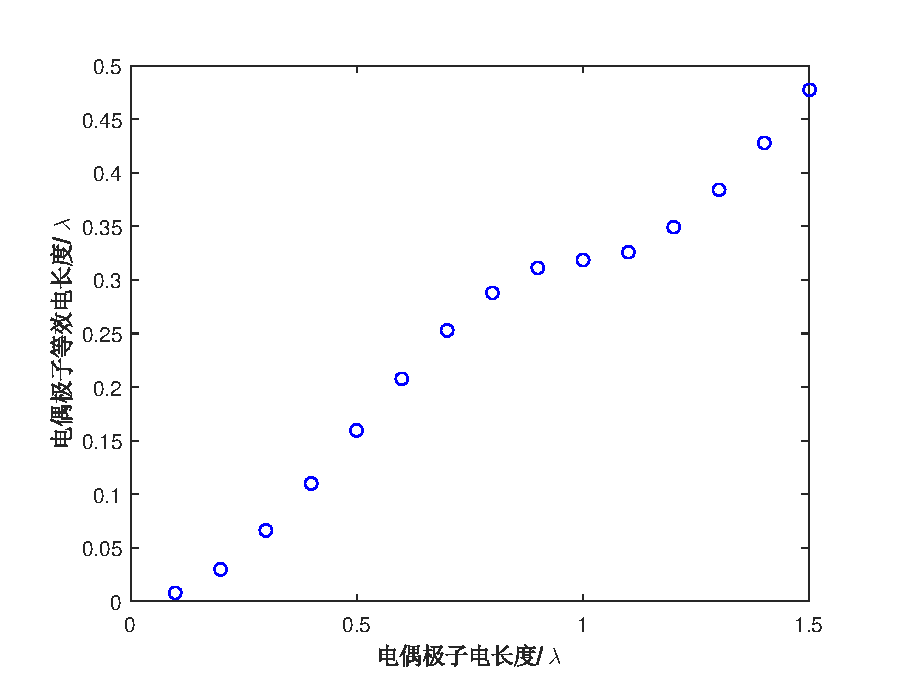
\includegraphics[width=10cm]{Dipole_Eq_length.eps}
\caption{等效电长度} \label{fig:DP_EQ_L}
\end{figure}
\subsubsection{选做:电流为均匀分布时的方向图}
结果如图\ref{fig:DP_i0} ,同图\ref{fig:DP}对比容易发现,在$L\le\lambda$时, 方向图相差不多,当$L>\lambda$方向图出现了明显差异,不考虑电流分布的方向图不会出现旁瓣.结果也恰好和教材上提到的,随着尺寸的增大.

易知,随着电偶极子尺寸的增大,电流分布的影响会愈发明显.
\begin{figure}[!ht]
	%\small
	\centering
	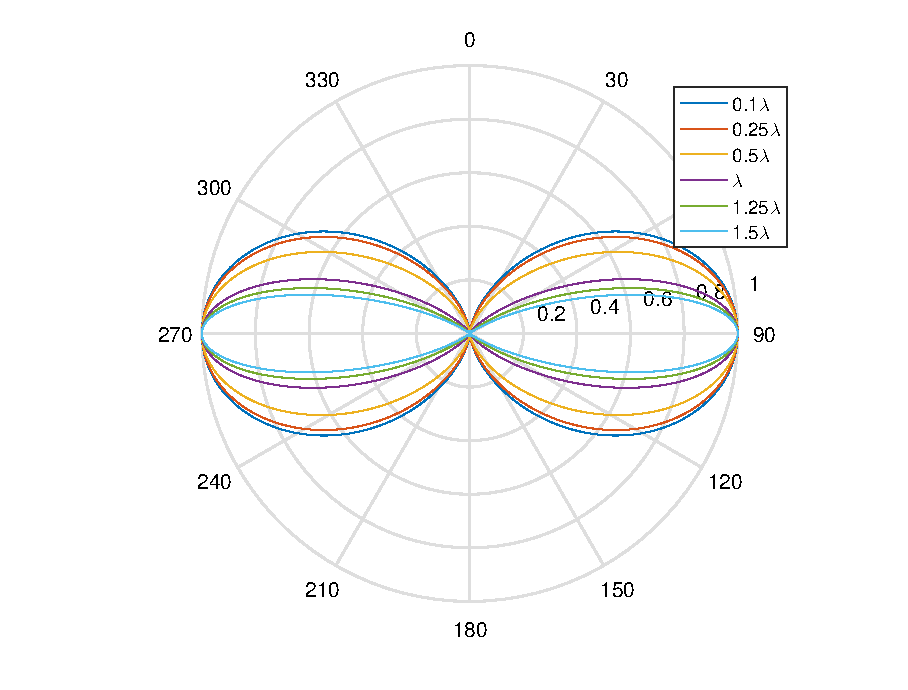
\includegraphics[width=10cm]{DipolePattern_i0junyun.eps}
	\caption{DipolePattern\_$\mathrm{I_0}$} \label{fig:DP_i0}
\end{figure}







\subsection{程序}
\noindent \textbf{绘制方向图主程序}
\begin{lstlisting}[language={matlab},keywordstyle=\color{blue!70},commentstyle=\color{red!50!green!50!blue!50},frame=shadowbox, rulesepcolor=\color{red!20!green!20!blue!20}] 
clear
close all

L=[.1,.25,.5,1,1.25,1.5];
BeamWidth=[];
temp='';
for i=1:length(L)
    BeamWidth(i)=Fun_DipolePattern(L(i));
    temp=num2str(L(i));
    legend(temp)   
    hold on 
end
legend('0.1','0.25','0.5','1','1.25','1.5')
view(90,-90)
figure
%当L=1.5时候, 编写的BeamWidth计算没有参考意义
BeamWidth(1,5)
plot(L,BeamWidth,'or')

\end{lstlisting}

\noindent \textbf{子程序}
\begin{lstlisting}[language={matlab},keywordstyle=\color{blue!70},commentstyle=\color{red!50!green!50!blue!50},frame=shadowbox, rulesepcolor=\color{red!20!green!20!blue!20}] 
function BeamWidth_3dB=Fun_DipolePattern(L,StepNum)
%归一化非dB的结果
%L是偶极子的电长度 略去lambda
%StepNum绘图精度,缺省时候为400
%返回值为BeamWidth_3dB
%lambda对方向图没有影响
if nargin<2
    StepNum=400;
end
    
theta=linspace(0,2*pi,StepNum);
fenzi=cos(pi*L*cos(theta))-cos(pi*L);
U=(fenzi./sin(theta)).^2;
U1=U/max(U);
polar(theta,U1)
%solve 3dB BandWidth
dB3=find(U1(1:StepNum/2)>=0.5);
BeamWidth_3dB=(max(dB3)-min(dB3))/StepNum*360;

end
\end{lstlisting}
\noindent \textbf{选做:计算等效电长度}
\begin{lstlisting}[language={matlab},keywordstyle=\color{blue!70},commentstyle=\color{red!50!green!50!blue!50},frame=shadowbox, rulesepcolor=\color{red!20!green!20!blue!20}] 
%计算电长度
clear
close all
for j=1:150
   L=1/10*j;
syms z
% I=I0*sin(k*L/2-k*z), 
%k l/2=pi*L 
% k z= 2*pi/lamad * lamada*L;
I=abs(sin(pi*L-2*pi*z));
vpa(int(I,z,0,L/2),6);
plot(L,vpa(int(I,z,0,L/2),6),'b.');
hold on
end
\end{lstlisting}
\noindent \textbf{选做:电流均匀分布}
\begin{lstlisting}[language={matlab},keywordstyle=\color{blue!70},commentstyle=\color{red!50!green!50!blue!50},frame=shadowbox, rulesepcolor=\color{red!20!green!20!blue!20}] 
%主程序
clear
close all
L=[.1,.25,.5,1,1.25,1.5];
BeamWidth=[];
temp='';
for i=1:length(L)
BeamWidth(i)=Fun_DipolePattern_i0(L(i));
temp=num2str(L(i));
legend(temp)   
hold on 
end
legend('0.1\lambda','0.25\lambda','0.5\lambda',
'\lambda','1.25\lambda','1.5\lambda')
view(90,-90)

%子函数
function BeamWidth_3dB=Fun_DipolePattern_i0(L,StepNum)
if nargin<2
StepNum=2000;
end
theta=linspace(0,2*pi,StepNum);
%sin(pi*L*cos(theta))*tan(theta);
U=(sin(pi*L*cos(theta)).*tan(theta)).^2;
U1=U/max(U);
polar(theta,U1)
end


\end{lstlisting}